\documentclass{scrreprt}
\usepackage{scrhack}
\KOMAoptions
{
  draft,
  DIV=calc, % this will calculate correct margins
  fontsize=12pt,
  listof=numbered,
}

\usepackage[english]{babel}

\usepackage[autostyle]{csquotes}

\usepackage[backend=biber,style=alphabetic]{biblatex}
\addbibresource{Bibliography.bib}

% Alternative to `Helvetica': TeX Gyre Heros
% Alternative to `Bookman Old Style': TeX Gyre Bonum
\usepackage{fontspec}
\setromanfont{TeX Gyre Bonum} % Enhanced version of `Bookman Old Style'.
\setmonofont{Consolas}
% \setsansfont{TeX Gyre Heros} % Replacement for Helvetica.

% Choose default font family.
%
% Options:
%   \rmdefault   Use the serif font family as default.
%   \sfdefault   Use the sans-serif font family as default.
%   \ttdefault   Use the monospace font family as default.
\renewcommand{\familydefault}{\sfdefault}

\usepackage{ifdraft}
\usepackage{amsmath}

\PassOptionsToPackage{draft}{graphicx}
\usepackage{graphicx}

\usepackage[toc,page]{appendix}

\usepackage{todonotes}
\newcommand{\tbd}[0]{\todo[inline, color=yellow!30]{\centerline{To Be Done}}}

\usepackage[acronym]{glossaries}
%!TEX root = ../Main.tex


%
% Acronyms
%

\newacronym{api}{API}{Application Programming Interface}
\newacronym{cpu}{CPU}{Central Processing Unit}
\newacronym{gpu}{GPU}{Graphics Processing Unit}
\newacronym{ram}{RAM}{Random Access Memory}
\newacronym{vram}{VRAM}{Video Random Access Memory}
\newacronym{gui}{GUI}{Graphical User Interface}
\newacronym{sdk}{SDK}{Software Development Kit}
\newacronym{2d}{2D}{two-dimensional}
\newacronym{3d}{3D}{three-dimensional}
\newacronym{dll}{DLL}{Dynamically Linked Library}

\newacronym{hlsl}{HLSL}{High Level Shading Language}
\newacronym{d3d9}{D3D9}{\gls{d3d} 9}
\newacronym{d3d10}{D3D10}{\gls{d3d} 10}
\newacronym{d3d11}{D3D11}{\gls{d3d} 11}
\newacronym{d3d12}{D3D12}{\gls{d3d} 12}

\newacronym{glsl}{GLSL}{OpenGL Shading Language}
\newacronym{spir}{SPIR}{Standard Portable Intermediate Representation}
\newacronym{spirv}{SPIR-V}{Standard Portable Intermediate Representation version `V'}
\newacronym{icd}{ICD}{Installable Client Driver}
\newacronym{ihv}{IHV}{Independent Hardware Vendor}

\newacronym{ps3}{PS3}{Sony PlayStation 3}
\newacronym{ps4}{PS4}{Sony PlayStation 4}
\newacronym{xbox360}{Xbox 360}{Xbox 360}
\newacronym{xbone}{Xbox One}{Xbox One}


%
% Glossary Entries
%

\newglossaryentry{c}
{
  name={C},
  description={The C programming language}
}

\newglossaryentry{cpp}
{
  name={C++},
  description={The C++ programming language}
}

\newglossaryentry{ccpp}
{
  name={C/C++},
  description={The C and C++ family of programming languages}
}

\newglossaryentry{csharp}
{
  name={C\#},
  description={The C\# programming language by \gls{ms}}
}

\newglossaryentry{python}
{
  name={Python},
  description={The Python programming language}
}

\newglossaryentry{host}
{
  name={host},
  description={The user of the Vulkan API}
}

\newglossaryentry{device}
{
  name={device},
  description={The GPU abstracted by the Vulkan API}
}

\newglossaryentry{application}
{
  name={application},
  description={The user of or the developer that uses the Vulkan API}
}

\newglossaryentry{driver}
{
  name={Vulkan implementation},
  description={The part of the Vulkan API that is opaque to the user, implemented in the hardware driver}
}

\newglossaryentry{vkloader}
{
  name={Vulkan Common Loader},
  description={The communication interface between Vulkan applications and \glspl{icd}}
}

\newglossaryentry{opengl}
{
  name={OpenGL},
  description={Open Graphics Library. A cross-platform \gls{api} for rendering in computer graphics with hardware acceleration}
}

\newglossaryentry{gles}
{
  name={OpenGL ES},
  description={OpenGL for Embedded Systems. Also known as OpenGL ES or GLES}
}

\newglossaryentry{dx}
{
  name={DirectX},
  description={Family of \glspl{api} for handling multimedia tasks on \acrfull{ms} platforms}
}

\newglossaryentry{d3d}
{
  name={Direct3D},
  description={\gls{dx} component used for 3D rendering in computer graphics}
}

\newglossaryentry{ms}
{
  name={Microsoft},
  description={Microsoft Corporation, commonly referred to as Microsoft or MS}
}

\newglossaryentry{windows}
{
  name={Microsoft Windows},
  description={Operating system developed and maintained by \gls{ms}}
}

\newglossaryentry{nvidia}
{
  name={NVIDIA},
  description={NVIDIA Corporation}
}

\newglossaryentry{amd}
{
  name={AMD},
  description={Advanced Micro Devices, Inc. (AMD)}
}

\newglossaryentry{intel}
{
  name={Intel},
  description={Intel Corporation, also known as Intel or intel}
}

\newglossaryentry{winapi}
{
  name={Windows \gls{api}},
  description={\gls{api} for \gls{windows} operating system calls}
}


\usepackage{xcolor}
\definecolor{CodeComment}{gray}{0.4}
\definecolor{CodeKeyword}{rgb}{0.0,0.0,0.8}
\definecolor{CodeString}{rgb}{0.0,0.3,0.0}

\usepackage{listings}
\lstdefinestyle{MyCpp}
{
  language=[11]C++,
  % backgroundcolor=\color{backcolour},
  commentstyle=\color{CodeComment},
  keywordstyle=\color{CodeKeyword},
  numberstyle=\ttfamily\color{CodeComment},
  stringstyle=\color{CodeString},
  basicstyle=\ttfamily,
  breakatwhitespace=false,
  breaklines=true,
  captionpos=b,
  keepspaces=true,
  numbers=left,
  numbersep=5pt,
  showspaces=false,
  showstringspaces=false,
  showtabs=false,
  tabsize=2
}
\lstset{style=MyCpp}

\usepackage{hyperref}
\hypersetup{
  colorlinks,
  final,
  bookmarksnumbered,
  citecolor=black,
  filecolor=black,
  linkcolor=black,
  urlcolor=black
}

\usepackage[nopar]{lipsum}
\setlipsumdefault{1}


\title{Evaluating the Resource Management Possibilites of the Vulkan Graphics API
  \todo[inline, color=red!64]{\centerline{DRAFT}}
}

\date{\today}
\author{Manuel Maier}

\begin{document}
  %
  % Title Page
  %
  \pagenumbering{gobble}
  \maketitle


  %
  % Blank page for physical notes, name entries, etc.
  %
  \newpage
  \null
  \pagenumbering{gobble}

  %
  % Abstract and acknoledgements.
  %
  %!TEX root = ../Main.tex

\ifthenelse{\boolean{hdm}}
{
\chapter*{Kurzfassung}
\label{Abstract_de}
  Dies ist die Kurzfassung.
  \todo[inline]{Will be composed once the English version is complete.}


\newpage
}
{}

\chapter*{Abstract}
\label{Abstract}
  In recent years, consumer graphics hardware has changed considerably.
  In the past, the hardware consisted only of fixed-function components that performed the necessary computations in a massively parallel manner to transform three-dimensional data to an image displayed on a screen.
  At the same time, APIs to graphics hardware were developed.
  As hardware design changed over the years, mainly to improve on performance, it has also become more generalized and accessible to other kinds of computational tasks\todo{Add ``than computer graphics''?}.
  Traditional APIs had to adjust to these design changes while maintaining compatibility to previously supported designs at the same time.
  This led to an increase in driver complexity, ultimately impacting performance in a negative way.
  New graphics APIs were designed to match recent hardware more closely, one of which is the Vulkan graphics API.

  In this work\todo{Use ``thesis'' or ``document'' instead of ``work''?}, the Vulkan graphics API is presented in three stages.
  At first, an overview of the API itself is provided.
  Afterwards, general instructions on how to set up an environment for developing Vulkan applications are given.
  And finally, the fundamentals of rendering an image using Vulkan are presented with the aid of simplified, prototypical examples.

  %!TEX root = ../Main.tex

\chapter*{Acknowledgements}
\label{cha:Acknowledgements}

These are my acknowledgements.

\todo[inline]{Make proper sentences below.}

\paragraph{Stefan Radicke}
  supervision.
  Lorem ipsum dolor sit amet, consectetuer adipiscing elit. Aenean commodo ligula eget dolor. Aenean massa. Cum sociis natoque penatibus et.

\paragraph{Patrick Bader}
  supervision.
  Lorem ipsum dolor sit amet, consectetuer adipiscing elit. Aenean commodo ligula eget dolor. Aenean massa. Cum sociis natoque penatibus et.

\paragraph{Hannes Pernpeinter}
  discussion, proof-reading.
  Lorem ipsum dolor sit amet, consectetuer adipiscing elit. Aenean commodo ligula eget dolor. Aenean massa. Cum sociis natoque penatibus et.

\paragraph{Christopher Manthei}
  discussion, proof-reading, experience.
  Lorem ipsum dolor sit amet, consectetuer adipiscing elit. Aenean commodo ligula eget dolor. Aenean massa. Cum sociis natoque penatibus et.

\paragraph{Benjamin Thaut}
  ???.
  Lorem ipsum dolor sit amet, consectetuer adipiscing elit. Aenean commodo ligula eget dolor. Aenean massa. Cum sociis natoque penatibus et.

\paragraph{Maria Floruß}
  rubber-ducking, proof-reading, support, help with illustrator.
  Lorem ipsum dolor sit amet, consectetuer adipiscing elit. Aenean commodo ligula eget dolor. Aenean massa. Cum sociis natoque penatibus et.



  %
  % Table of Contents
  %
  \newpage
  \pagenumbering{roman}
  \tableofcontents
  \newpage


  %
  % Chapters
  %
  \pagenumbering{arabic}
  %!TEX root = ../Main.tex

\chapter{Introduction}
\label{cha:Introduction}
  \todo[inline]
  {
    Brief introduction of computer graphics. One of the biggest problems: Performance. Especially with virtual reality.

    Maybe mention the author's (that's me!) bias towards game development.

    Mention target audience requirements.

    Explain shader stages of modern graphics hardware somewhere in this chapter.
  }

  % The field of computer graphics poses many challenges.

  % Data is consumed by a pipeline and transformed by complex algorithms, resulting in another set of data that is used in further processing. This transformation process is usually referred to as ``rendering''. In its most simple form, the output of the rendering process is used to present a graphical representation of the input data to the user, typically via a computer monitor peripheral device.

  % Computer graphics is an area of computer science that has many disciplines. Examples are \glspl{gui}, computer vision, sprite graphics, and \gls{3d} modelling. Most relevant to this paper is \gls{3d} computer graphics. \todo{Mention how Vulkan is not only suited for \gls{3d} graphics?} The most typical use case in \gls{3d} computer graphics is to process data, usually three-dimensional geometric data, in order to produce a 2D image which is then presented to the user with the help of a computer monitor. This processing of data is referred to as \textit{3D rendering} or simply \textit{rendering}.

  % While 3D rendering can be implemented in software, special hardware called a \gls{gpu} can be used instead to achieve better performance. The need for such hardware already indicates one of the greatest challenges in 3D computer graphics: performance. The amount of data involved in 3D rendering can become quite large. As an example, assume the following:

  % \todo{Explain what a Vertex is and how graphics hardware produces faces etc.}

  % The aforementioned three-dimensional geometric data can be given in many different ways. The ideal way of representing specific data depends on the use case and the entire 3D graphics pipeline.

  % For the sake of illustration, let's assume a data set that consists only of 3D vertices. In this example, each vertex only has a position defining the absolute location of the vertex in 3D space. This position value is stored as a vector of three floating point numbers. Typically, such floating point numbers are standard IEEE floating point numbers (as per IEEE 754), taking up 32 bits or 4 bytes of memory. Thus, each vertex takes up $3*4 = 12$ bytes of memory.

  % On desktop systems, applications typically don't access the graphics hardware directly. They instead communicate with a driver that manages hardware access. Communication between an applicatin and the driver is done via an \gls{api}. Figure \ref{fig:AppApiDriverOverview} visualizes this relationship. Ideally, the application does not need to know which specific driver it is communicating with as long as the driver is compliant to the \gls{api} specification. This abstraction decouples the application from the hardware and enables it to run on systems with different hardware configurations without altering the application itself. It also enables hardware vendors to manipulate or even reject operations requested by the application, typically to enforce some user-specified global settings. \todo{Explain what kind of settings? Maybe give an example?}

  \begin{figure}
    \centering
    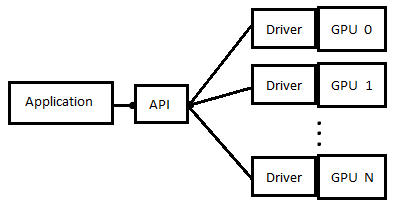
\includegraphics{Main/Images/Application_API_Driver_Overview}
    \caption{Interaction between the application and the hardware via the API.}
    \label{fig:AppApiDriverOverview}
  \end{figure}

  \todo[inline]{Talk about different kinds of graphics \glspl{api} on different systems (D3D, OpenGL on desktop, maybe Metal for OSX, and special \glspl{api} on consoles.)}


  \section{High Level Graphics Workflow}
    \label{sec:GraphicsWorkflow}
    \todo[inline]
    {
      General overview of the stages several resources (vertices, textures, etc.) have to go through.

      Explain the fixed function pipeline.
    }

    \missingfigure{Visualize data flow of data between shader stages.}
    \tbd


  \section{Motivation for a new Graphics API}
    \todo[inline]{Basically write why Vulkan is needed.}

    Graphics hardware is changing rapidly through the years and is highly specialized to do computational work in a massively parallel manner. This makes it not only suitable for graphics computation, but also for general-purpose parallelization of working with large sets of data. These \glspl{api} have grown with the hardware, constantly adapting to it, adding new versions that support different kinds of features and provide different kinds of extensions while maintaining backwards compatability as much as possible. This lead to very complicated \glspl{api} that was getting harder and harder to understand with each new release, especially for beginners.

    \todo[inline]{It might be too obvious that the paragraph above refers to OpenGL. Maybe just make it OpenGL-specific. Would still need to explain why Vulkan is not as abstract as OpenGL. Parts of this is explained below.}

    But not only graphics and compute hardware has changed. The drivers accompanying the hardware also have to stay backwards compatible. They hide and abstract a lot of the low-level functionality that is needed to work properly with the hardware. This abstraction means that the application developer has less control over what is actually done with the data fed to drivers. Since drivers rarely get information about the exact intent of what the developer plans to do with the supplied data, they have to implement heuristics to decide the best course of action.

    This level of abstraction has been criticized by many professional developers over the years, demanding for more low-level control\todo{Reference something here. A paper, in the best case.}. On gaming consoles, low-level control of the hardware was always required, except for Microsoft platforms where the \gls{d3d} technology has always been in use. This meant that console developers were already used to thinking about data flow on a low level and work very closely with the hardware.

    Another aspect is the advent of multi-core CPUs for personal computers in the mid 2000's. Multithreading has become common in CPU programming to achieve better performance. Older graphics \glspl{api}, however, were designed to run on a single thread all the time. Even though these \glspl{api} provide limited support for multithreading by now, they were still originally not designed for it, making it rather difficult to fully utilize multicore performance.

    \todo[inline]{Talk about new \glspl{api} such as D3D12, Mantle, Metal, and also talk about consoles (no specs) that all adress these problems.}


  \section{The Vulkan Graphics and Compute API}
    \todo[inline]{What does it do. Where does it come from. What are people expecting from it. Cross-platform nature (in comparison maybe to PS4's libGNM made specifically for PS4 hardware).}

    \todo[inline]{Insert missing references.}
    The Vulkan \gls{api} was designed by the Khronos Group in collaboration with many industry representatives, including Valve Coroporation, AMD, NVIDIA. Version 1.0 of the Vulkan specification was released on the 16th February in 2016. It was designed to provide low-level control to the developer when interacting with graphics and compute hardware.

    Vulkan was designed with a variety of goals in mind.

    \begin{itemize}
      \item Cross-platform
      \item Keep driver complexity at a minimum
      \item Less driver-side CPU overhead
      \item Enable developers a lot of control over the hardware.
      \item Consistent API
    \end{itemize}

    There are many different kinds of hardware configurations today, ranging from high-end gaming systems to mobile platforms such as smartphones. Vulkan is designed to be used with all of these systems. There will be no special version of Vulkan dedicated to embedded systems as was the case with \gls{gles}.

    As a result of striving for less driver overhead, Vulkan also provides the possibility of reducing CPU and GPU power consumption. The driver implementation will have to make fewer guesses of what the host application is trying to do. It is up to the application developer to tell the Vulkan driver exactly what needs to be done. This way the driver only does as much work as it needs to function properly and less power will be consumed. Hardware vendors will also have an easier time providing robust drivers with less bugs due to reduced complexity.

    Another advantage of Vulkan, being a new API built without worrying about backwards compatability, is the chance of designing a new and consistent API so developers will have an easier time creating applications. For more information about the API structure and common patterns in Vulkan, see chapter \ref{cha:VulkanOverview}.

    Version 1.0 of Vulkan was not entirely built in-house at Khronos Group but is in part based on components of AMD's Mantle API, which was donated to the Khronos Group.


    \subsection{Vulkan Competitors}
      \todo[inline]{OpenGL, Direct3D11, Direct3D12, libGNM (PS4), OpenCL}

      Other \glspl{api} exist that are direct competitors to Vulkan.

      \gls{opengl} is Vulkans predecessor and provides a higher level of abstraction from the hardware. It is a very successful API running on several different platforms with varying hardware configurations. Due to its level of abstraction, \gls{opengl} drivers are very complex and do a significant amount of work on the CPU in order to match abstract commands to the hardware.

      Special flavors of \gls{opengl} exist, such as \gls{gles}, which is a subset of \gls{opengl} to enable hardware-accelerated graphics processing on embedded systems such as smartphones and tablets.

      The \gls{d3d} family of \glspl{api} is developed by Microsoft and only supports Microsoft platforms such as the Windows operating system or the Xbox gaming console. The most recent versions of \gls{d3d} are \acrlong{d3d11} and \acrlong{d3d12}. \acrlong{d3d11} provides a higher level of abstraction from the hardware, not unlike \gls{opengl}. It has been around since the release of Windows 7 in 20??\todo{date}. \acrlong{d3d12}, the latest revision of the \gls{d3d} specification released in 2015\todo{exact date?}, is comparable to Vulkan in terms of of hardware abstraction. It provides much more control to the developer over the hardware.

      \todo[inline]{Mac OS X: Metal}

      \todo[inline]{Gaming console graphics libraries.}

      \todo[inline]{OpenCL as compute API}


  \section{Document Structure}
    \todo[inline]{The structure and content of this document.}

    \tbd

  %!TEX root = ../Main.tex

\chapter{Vulkan API Overview/Workflow}
\label{cha:VulkanOverview}
  \todo[inline]
  {
    The Vulkan Graphics \acrfull{api} workflow, object creation, patterns (vkCreate/vkDestroy, vkAllocate/vkDeallocate), synchronization.

    Listing and short explanation of Vulkan components such as buffers, images, command buffers.

    Note that when talking about a ``device'', a logical device is meant. When referring to the actual hardware component the term ``physical device'' will be used.

    Mention queues and queue families somewhere before the Synchronization section.
  }
  \todo[inline]{Refer to Vulkan spec.}

  This chapter provides an overview of the Vulkan API and explains some concepts in more detail. In some places an abbreviated form is used when referring to several Vulkan commands at once, e.g. \lstinline{vkPlaceholder*} would refer to all Vulkan commands that begin with the character string ``vkPlaceholder'', e.g. \lstinline{vkPlaceholderCommand}. The asterisk is used as a wildcard character.

  Vulkan uses the terms ``host'' and ``device'' to refer to the CPU and GPU, respectively, when describing data flow or memory visibility. These terms will be used in this chapter as well with the same meaning.

  \section{Workflow and Patterns}
  \label{sec:WorkflowAndPatterns}
    The Vulkan API was designed to be consistent and explicit. Many patterns can be found in the Vulkan code style that make it easier for the developer to use the API effectively. This section is a walkthrough of the basic steps that need to be taken to set up a Vulkan graphics pipeline to present an image to a display.

    Vulkan makes use of handle types to allow the developer to track objects created with the API. The first object that has to be created is a Vulkan instance. The Vulkan instance can be used to query available physical devices that provide Vulkan support. These physical devices can be queried for certain capabilities, such as supported image formats and hardware features, to aid in deciding which physical device to use for the application. A physical device can subsequently be used to create a logical device, or just device. The number of devices created from a physical device is not limited. When a device is create, all queues associated with it are created as well. This is why there is no \lstinline{vkCreateQueue} but rather \lstinline{vkGetQueue} command. Among other things, devices are used to allocate Vulkan objects or GPU memory. Changes made on Vulkan objects do not have global side-effect observable with the regular Vulkan API. However, drivers and Vulkan layers or extensions are free to modify their own state across Vulkan object boundaries.\todo{Redundant sentence? This should be a given.}

    \todo[inline]{Describe/mention GPU queues in the introduction chapter.}

    Once a device handle has been acquired the developer can create a swapchain to establish a connection between a specific queue on the device and a platform specific presentation engine. A swapchain contains a number of ``presentation images'' the contents of which are produced by the graphics pipeline. These ``presentation images'' are regular Vulkan image objects in a specific format.

    In order to produce images for the presentation engine to consume via the swapchain, a graphics pipeline needs to be created. This graphics pipeline consists of one or more render pass objects that hold information about how to complete a rendering step. Examples of the render pass state that has to be set is the used pipeline stages, such as vertex or fragment shader stages or compute shader stages, as well as setting framebuffer attachments. Render passes can be organized into subpasses which can be set up to depend on other subpasses, e.g. for post-processing.

    With a graphics pipeline in place, command buffers can be used to record rendering commands such as copying device memory to another location or issueing drawing commands. In order to record command, the command buffer needs to set into recording mode. For more information about command buffers, refer to chapter~\ref{cha:GpuResources}.

    \todo[inline]{Put the following into a subsection?}

    Creating Vulkan objects is done by calls to \lstinline{vkCreate*} commands which take a pointer to \lstinline{Vk*CreateInfo} structures and return a handle to the created object. These info structures contain parameters used by the creation command to create the requested type of Vulkan object. The contents of such info structures are specific to each creation command and require the developer to consult the Vulkan specification in order to provide correct input data. Destroying Vulkan objects is done by passing an object handle to those \lstinline{vkDestroy*} commands that exactly correspond to the \lstinline{vkCreate*} command that created the object in the first place. The commands \lstinline{vkCreateBuffer} and \lstinline{vkDestroyBuffer} are examples for this.

    When Vulkan objects are allocated from memory pools, or directly from device memory, calls to \lstinline{vkAllocate*} commands have to be made. These commands are accompanied by \lstinline{vkFree*} commands that return resources to their origin where they originally were acquired from. The general rule is that all objects allocated from pools are released as soon as the pool itself is released. Using Vulkan objects that are released results in undefined behavior, similar to using deallocated memory in C/C++.

    Unlike other APIs, Vulkan does not do any object tracking or reference counting to manage object life times. It is the responsibility of the developer to destroy or free Vulkan objects at the appropriate times, i.e. when they are no longer in use and will not be used in the future by either the host or the device.

    Vulkan objects are not designed to be thread-safe. This means that accessing or modifying a Vulkan object from more than one thread at once can lead to race conditions or other undesirable behavior. It is the responsibility of the developer to employ proper synchronization mechanisms on the host to ensure Vulkan objects are never accessed concurrently.

  \section{Layers and Extensions}
  \label{sec:LayersAndExtensions}
    \todo[inline]{Layers are instance-only, extensions are both on the isntance-level as well as the device-level.}

    Vulkan is designed to be extensible by thirdparty developers. The two mechanisms provided are called layers and extensions.

    A layer in Vulkan can be thought of as an observer to the API calls done by the developer. It does not add new types or commands the developer can use directly.\todo{Illustration of Vulkan with some layers between it and the user}\todo{Elaborate more to make it crystal clear. Make sure to mention no layers are needed.}

    The LunarG SDK, for example, comes with a set of layers to validate usage of the Vulkan API. This is extremely useful during development as it allows the developer to focus on their code rather than the perfect use of the Vulkan API. It should also be noted that bare Vulkan, without any validation layers enabled, does not do any error checking. When the developer passes an invalid combination of flags to some Vulkan function, it is undefined behavior and has to be corrected by the developer.

    Layers can only be created on the instance-level. Until version x.x.x.x \todo{Find out the exact version.}, the developer was able to create device-level layers, but these are deprecated in Vulkan version x.x.xx.x by now.

    \todo[inline]{Pull out neutral descriptions of layers/extensions and put the examples in their own paragraph.}

    As opposed to layers, extensions are able to provide new or add to existing functionality. The motivation for extensions is to keep the Vulkan core functionality small and provide specific functionality via such extensions. In fact, the Khronos Group itself provides built-in extensions for both common and platform specific functionality. An example of an extension that adds platform independent functionality is the \lstinline{VK_KHR_swapchain} extension. It adds several types and commands to create and interact with a swapchain. The concept of a swapchain itself is independent of the platform but it requires the help of platform specific functionality in order to work. On Windows platforms, for example, the developer needs to enable the \lstinline{VK_KHR_win32_surface} extension in order link a swapchain to a Win32 window. From a developer's perspective, they do not have to care about distinguish between platforms when creating a swapchain but they do have to when creating and connecting the swapchain to a surface.

    Extensions can be enabled on both instance-level and device-level. Instance-level extensions provide functionality that is generally independent of the hardware.

    An example for an instance-level extension is \lstinline{VK_EXT_debug_report}. It enables the developer to provide a callback function that is used by Vulkan layers or extensions to communicate with the developer. If validation layers are enabled, this is how they would tell the developer about any validation concerns or violations. An example for a device-level extension is the aforementioned \lstinline{VK_KHR_swapchain} extension. Not all physical devices have to be capable of rendering graphics images. In the end it is up the extension author on which level they provide their extension.

  \section{Memory Management and Resources}
  \label{sec:MemoryManagement}
    \todo[inline]{
      Allocate memory separately and then binding it to resources. Decoupled on purpose for custom management and reuse.

      Introduce buffers, images, global memory and command buffers.


      Command buffers have their own state. Used with vkCmd commands. Are submitted to a queue. Submissions can be executed out of order.

      Investigate: execute commands out of order within the same submission? If no barrier is present, of course.
    }

    Memory management is an important topic in Vulkan.

    \tbd

  \section{Pipelines and Render Passes}
  \label{sec:RenderPasses}
    \todo[inline]
    {
      Distinction between graphics and compute pipeline.

      Pipeline consists of a render pass that may have sub-passes. Pipeline inheritance.

      Pipeline Cache and optimization by storing it on disk.
    }
    \tbd

  \section{Shader Language: SPIR-V}
    \todo[inline]{\acrfull{spir-v}}

    Shader programs are supplied to Vulkan in \acrfull{spir-v} format. \acrshort{spir-v} is a high-level graphics and parallel compute programming language provided in a binary format. The specification is entirely maintained by the the Khronos Group.

    \todo[inline]{Mention tools for SPIR-V.}

    \todo[inline]{Par below needs expanding. Goal is to describe why SPIR-V is a good thing and how people benefit from it.}
    One might wonder why the Khronos Group chose to only support an intermediate representation for shader programs instead of using something like the \acrfull{glsl} that is already in wide-spread use. \todo{Mention OpenGL supports SPIR-V now as well?}

  \section{Synchronization}
    \todo[inline]{Describe what Vulkan offers and discuss the individual use-cases as well as their performance impact.}

    \todo[inline]{Maybe reduce the use of `Vulkan was designed to' throughout the document?}
    Vulkan was designed to run concurrently. Synchronization is the responsibility of the application (mainly). in order to do so, Vulkan provides four types of synchronization primitives: fences, semaphores, events, and barriers. These synchronization primitives can be used to insert execution and memory dependencies in various circumstances.

    \todo[inline]{Explain execution and memory dependencies here?}

    \subsection{Fences}
    \label{sub:Fences}
      A fence is a synchronization primitive used to determine the execution status of submitted operations executed on a queue. Such a fence can only be in one of two states: not signaled and signaled. The status of a fence is visible to the host. The device itself does not use the status of a fence directly.

      In practice, a fence is most commonly used with the \lstinline{vkQueueSubmit} command, which is used to submit work to a device queue that were previously recorded to command buffers. The application can query the fence for its status using \lstinline{vkFenceGetStatus} which determines whether the fence was signaled or not. Waiting for a fence to be signaled essentially means waiting for all of the submitted work on the queue to be finished.\todo{Make clear it's only the work that was given in the same queue submission as the fence}{} In order to wait for a fence to be signaled in a blocking\todo{Sugarcoat the term `blocking' a bit?}{} fashion the \lstinline{vkWaitForFences} command is used.

    \subsection{Semaphores}
    \label{sub:Semaphores}
      A semaphore is similar to a fence, as discussed above in \ref{sub:Fences}\todo{Should I omit this?}, except that its status is only visible to the device. It can be used to synchronize operations within the same and between different device queues.

      The most common use case for Vulkan semaphores in a graphics application is when presenting swapchain images to the presentation engine. First, the commands to create the final image have to be recorded to a command buffer. This command buffer then needs to be submitted to a queue in order to be executed. When submitting to the queue, a semaphore can be provided that will be signaled once the queue has finished executing all submitted commands. The same semaphore can be used when issuing the swapchain presentation command. When everything is set up like this, the presentation engine will effectively wait for the commands to produce the final image and then present it as fast as possible.

      Note that a fence can be used to achieve the same results except that it would require the host to actively wait for the queue to finish executing, stalling any other CPU operations that could have been executed in that time. Using the semaphore in this case will result in better performance.

    \subsection{Events}
    \label{sub:Events}
      Events are used to synchronize from host to device or from device to device in a bidirectional manner. Like semaphores and fences, events are in either a signaled or in a not-signaled state. Events are inserted into command buffers in order to allow the device to signal them. This allows for more fine-grained synchronization between commands and to signal command completion the host. Unlike a fence, an event can be inserted at any point in the command buffer stream and thus can be used to query for synchronization without requiring that all commands in the submitted command buffer have completed execution.

      The way events work could be taken advantage of in a batch resource transformation scenario. Imagine there are an arbitrary number of images in an application that need to be transformed in some way that is expensive to compute. These transformations could be issued into a single command buffer, inserting a completion event between transformation commands. After submitting this command buffer to the queue, the application can periodically query for completion of the individual transformation commands without the need to wait for the entire submission to finish by using fences or semaphores.

      It must be noted that events are only allowed to be insterted into command buffers that are all submitted to the same queue. This makes them unuseful if cross-queue synchronization is requried.

    \subsection{Barriers}
    \label{sub:Barriers}
      Barriers are used exclusively with commands recorded to command buffers. There are two kinds of barriers in Vulkan. The first kind is called an execution barrier which are used to create explicit dependencies on the completion of specific commands. The second kind is called a memory barrier which are used to depend on memory to be present in a specific form. Both kinds of barriers are combined in Vulkan as a pipeline barrier.\todo{Add illustration of floating commands above and below a pipeline barrier.}

      \begin{figure}
      \caption{Illustration of a pipeline barrier insterted between commands in a command buffer.}
      \centering
      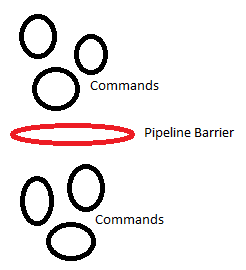
\includegraphics{Main/Images/PipelineBarrier}
      \label{fig:PipelineBarrier}
      \end{figure}

      By inserting a memory dependency, the application indicates to the API that all memory operations need to be finished on a specified resource or memory region once the inserted barrier has been reached. Otherwise all following commands are not able to begin executing. Analogously, an execution dependency requires all previous commands to have finished execution before starting to execute other commands inserted after the barrier.

      There are three types of memory barriers in Vulkan: Global memory barriers, buffer memory barriers, and image memory barriers.

      \subsubsection{Global Memory Barriers}
        \todo[inline]
        {
          Investigate: Are these truly global memory barriers? The spec reads ``applies to memory accesses involving all memory objects that exist at the time of its execution'' which seems very heavyweight.
        }
        Global memory barriers introduce a dependency to all memory objects that exist at the time of execution of the barrier. All prior memory access operations, whether they are read or write operations, must have finished before the barrier finishes execution.

        Such heavy-weight memory dependencies are not needed if the memory in use is entirely cache coherent. In other words, if the rest of the system ensures that all caches are flushed at appropriate times, memory accesses from other parts of the system will be consistent and up-to-date\todo{Double-Triple-Check whether this is actually correct.}.

      \subsubsection{Buffer Memory Barriers}
        Buffer memory barriers introduce a memory access dependency on a specific region of memory associated with a buffer object. That region may encompass the entire buffer and is specified in terms of an offset, relative to the beginning of the buffer, and a size value.

        This kind of barrier can be used to transfer ownership of a buffer region to another queue family or to change access flags of that region. Transferring ownership of that buffer region to another queue family is only possible if this kind of operation has been enabled for that buffer at the time it was created. Access flags are used to control how the buffer region is accessed. They could be used to make the memory region read-only, for example, or enable host access for it.

      \subsubsection{Image Memory Barriers}
        Image memory barriers are similar to buffer memory barriers. They can be used to transfer ownership image regions to another queue family, modify access flags, and to change the image layout. An image region is specified differently from a buffer region of the fact that images need not be stored linearly in device memory\todo{Refer to wherever image tiling is explained}.

        Transferring ownership of an image region is only possible if the image was set up correctly at creation time. Modifying access flags has the same effect as with modifying access flags on a buffer region.

        Changing the layout of the image is an important operation on Vulkan images. For example, it is required for swapchain images in order to be presentable. The presentation engine requires swapchain images to be in a specific layout when presenting them so the application must ensure that the image has that specific layout before attempting to issue the presentation command. Since the presentation layout is only meant for use by the presentation engine, the application has to use another image memory barrier to change the layout into something that can be used by the host application.

    % Fences are

    % There are semaphores, fences, and pipeline barriers.

    % Fences are used to ... and can be waited on using the function \lstinline{vkWaitFences}. Fences are like

    % \todo[inline]{Illustrate a pipeline barrier?}
    % As mentioned in section \ref{sec:CommandBuffers}, commands recorded in a command buffer can be executed out-of-order\todo{Is this \textbf{really} true?} on the queue it is submitted on. The developer can explicitly synchronize
    % Pipeline barriers are used to synchronize execution state and
    % Pipeline barriers are used to ensure all memory operations have finished at a certain point in the pipeline. These barriers are inserted into a command buffer using the \lstinline{vkCmdPipelineBarrier} command. A  common use-case is transitioning a Vulkan image from one layout to another, e.g. from a layout optimized for presentation purposes to a layout optimized for

  \section{Interaction with the Operating System}
    \todo[inline]
    {
      Windowing system, specific Vulkan extensions per OS.

      \textbf{Kill this section?}
    }

  %!TEX root = ../Main.tex

\chapter{Vulkan GPU Resources}
\label{cha:GpuResources}
  \todo[inline]
  {
    Different kinds of resources for different kinds of operations. These have been introduced in the previous chapter already and will now be explained in more detail.
  }

  \todo[inline]
  {
    Possible pattern per section: What is the resource used for $\rightarrow$ How is it allocated $\rightarrow$ Discuss synchronisation issues.
  }

  \tbd

  \section{Images and Buffers}
    \todo[inline]{Difference and why it matters.}

    \tbd

  \section{Command Buffers}
    \todo[inline]{Record commands into buffers that are uploaded to the gpu to be replayed there.}

    \tbd

  \section{Shaders and Pipelines}
    \todo[inline]
    {
      Data flow between CPU and GPU. Data flow within the GPU through shaders.

      Descriptor pool/layout/set/set-layout
    }

    \tbd

  %!TEX root = ../Main.tex

\chapter{Resource Management Techniques}
\label{cha:ResourceManagementTechniques}
  \todo[inline]{Discuss what to do in certain situations, e.g. when uploading image data using a staging buffer.}

  \lipsum

  %!TEX root = ../Main.tex

\chapter{Evaluation}
\label{cha:Evaluation}
  \todo[inline]{Present and discuss preformance measurement results.}

  \lipsum

  %!TEX root = ../Main.tex

\chapter{Conclusion}
\label{cha:Conclusion}
  \todo[inline]{API quality. Explain and discuss why the API is called `modern', `highly efficient', and `explicit'.}
  \todo[inline]{Highly active development. LunarG provides more and more improved layers with each release.}
  \todo[inline]{Driver's are slow to keep up. No windows support from Intel for now.}
  \todo[inline]{Hard to learn, but probably worth it. Validation layers are awesome!}
  \todo[inline]{Mention Valve's plans for pipeline caches? Download pipeline caches when installing games.}
  \tbd



  \newpage
  \pagenumbering{Roman}


  %
  % Bibliography
  %
  \newpage
  \printbibliography[heading=bibintoc,title=Bibliography]
  \nocite{*} % Make sure to print all bibliography entries.

  %
  % Appendix
  %
  %!TEX root = ../Main.tex

\appendix


%
% List of Listings
%
\renewcommand\lstlistlistingname{List of Listings}
% \addcontentsline{toc}{chapter}{\lstlistlistingname}
\lstlistoflistings


%
% List of Figures
%
\listoffigures


%
% List of Tables
%
% \listoftables


% \chapter{Prototype Source Code}
%   \label{cha:PrototypeSourceCode}
%   \todo[inline]
%   {
%     Goals:\\
%     -- Refer to the disc that came with the thesis document.\\
%     -- Also refer to GitHub. Make sure the source code is in the MastersThesis repo.\\
%   }
%   \tbd


%
% Document Source Code
%
\chapter{Document Source}
  The sources of this document can be found on GitHub using the following \gls{url}.
  Published versions of this document can also be found there in the \textit{releases} section.
  \newline

  \noindent
  \url{https://github.com/Manuzor/MastersThesis}
  \newline

  \noindent
  The published version of this document is \lstinline{v1.0} and can be found using the following \gls{url}.
  \newline

  \noindent
  \url{https://github.com/Manuzor/MastersThesis/tree/v1.0}


%
% Prototype Source Code
%
\chapter{Prototype Source Code}
  During the development of this document, another project has been developed concurrently.
  The project is written in \gls{cpp} and uses the Vulkan graphics \gls{api}.
  It was mainly used for experimenting with Vulkan and everything closely involved.
  The project is only losely connected to this document but may still provide a valuable resource to the reader.
  \newline

  \noindent
  \url{https://github.com/Manuzor/VulkanExperiments}


\end{document}
